\section{Kvadratsætninger}
\noindent Hvis vi har et udtryk som vi gerne vil reducere, møder vi ofte noget på formen $(a+b)^2$. For at komme videre i vores udregning vil vi derfor gerne kunne omskrive sådanne udtryk så de bliver nemmere at reducere. Til at gøre dette introducerer vi kvadratsætningerne.

Vi husker at når vi ganger to parenteser sammen, så benytter vi følgende formel
\begin{align*}
(a+b)(c+d)=ac+ad+bc+bd,
\end{align*}
som vi får ved først at gange $a$ ind på begge elementer i den anden parentes og dernæst gange $b$ ind på de to elementer.

Hvis vi bruger denne regneregel får vi:
\begin{align*}
&(a+b)^2=(a+b)(a+b)=a^2+ab+ba+b^2=a^2+b^2+2ab \\
&(a-b)^2=(a-b)(a-b)=a^2-ab-ba+(-b)^2 = a^2+b^2-2ab\\
&(a+b)(a-b)=a^2-ab+ba-b^2 = a^2-b^2.
\end{align*}
Bemærk her, at $(-b)^2 \neq -b^2$ medmindre $b=0$, da $(-b)^2 = (-b)\cdot (-b)=(-1)\cdot b \cdot (-1) \cdot b = (-1)^2 \cdot b^2 = b^2$ og $-b^2 = (-1) \cdot b^2$.

Det giver os de tre kvadratsætninger, som kort kan skrives:
\begin{enumerate}
\item $(a+b)^2=a^2+b^2+2ab$.
\item $(a-b)^2=a^2+b^2-2ab$.
\item $(a+b)(a-b)=a^2-b^2$.
\end{enumerate}

\paragraph{Eksempler:}
\begin{enumerate}
\item Reducer $(x+y)^2+(x-y)^2-x^2-y^2$:
\begin{align*}
(x+y)^2+(x-y)^2-x^2-y^2 &= x^2+y^2+2xy + x^2+y^2-2xy - x^2-y^2 \\
&=x^2+y^2.
\end{align*}
\item Reducer $\frac{1}{a+b}+\frac{1}{a-b}$:

Ved at benytte brøkregnereglerne fra sidste kursusgang får vi
\begin{align*}
\frac{1}{a+b}+\frac{1}{a-b} &= \frac{a-b}{(a+b)(a-b)} + \frac{a+b}{(a+b)(a-b)} \\
&= \frac{a-b+a+b}{(a+b)(a-b)} \\
&=\frac{2a}{a^2-b^2}.
\end{align*}
\item Reducer $\frac{2x^2+2-4x}{2x^2-2}$:

Vi ser ved hjælp af vores kvadratsætninger at
\begin{align*}
&2x^2+2-4x = 2(x^2+1-2x) = 2 (x-1)^2 \\
&2x^2-2 = 2(x^2-1) = 2(x-1)(x+1).
\end{align*}
Hvis vi indsætter dette og reducere, får vi
\begin{align*}
\frac{2x^2+2-4x}{2x^2-2} = \frac{2 (x-1)^2}{2(x-1)(x+1)} = \frac{x-1}{x+1}.
\end{align*}
\end{enumerate}

\paragraph*{Afstandsformlen:} Vi husker Pythagoras Sætning der siger at for en retvinklet trekant med sidelængderne $a,b,c$ hvor $c$ er hypotenusen, gælder der:
\begin{align*}
a^2+b^2=c^2.
\end{align*}
Ved at benytte Pythagoras Sætning får vi at afstanden $c$ mellem to punkter $P$ og $Q$ i et koordinatsystem som i Figur~\ref{fig:1lec} 
\begin{figure}[!htbp]
  \pgfplotsset{width=0.5\textwidth,compat=1.11}
  \centering
  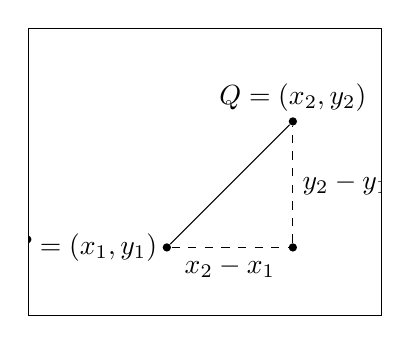
\begin{tikzpicture}
  \begin{axis}[ 
    xmin=-0.1,
    xmax=2.7,
    ymin=0.5,
    ymax=1.7,
    axis equal,
    %axis lines=middle,
 ticks=none,
xlabel={},
ylabel={},
  ]
\node[circle,fill,inner sep=0pt,minimum size=3pt] (P) at (1,0.5) {};
\node[below,left] at (1,0.5) {$P=(x_1,y_1)$};
\node[circle,fill,inner sep=0pt,minimum size=3pt] (Q) at (2,1.5) {};
\node[above] at (2,1.5) {$Q=(x_2,y_2)$};
\node[circle,fill,inner sep=0pt,minimum size=3pt] (R) at (2,0.5) {};
\draw (P)--(Q);
\draw[dashed] (P)--(R)--(Q);
\node[below] at (1.5,0.5) {$x_2-x_1$};
\node[right] at (2,1) {$y_2-y_1$};
%\draw (1,1) circle [radius =sqrt(2)]; 
\end{axis}
 \end{tikzpicture}
  \caption{Afstanden mellem $P$ og $Q$.}
  \label{fig:1lec}
\end{figure}
er givet ved
\begin{align*}
(x_2-x_1)^2+(y_2-y_1)^2=c^2.
\end{align*}

\paragraph{Cirklens ligning:}
Ved at bruge afstandsformlen kan vi nu opstille en ligning for en cirkel med centrum i punktet $(a,b)$ og med radius $r$, som i Figur~\ref{fig:2lec}.
\begin{figure}[!htbp]
  \pgfplotsset{width=0.5\textwidth,compat=1.11}
  \centering
  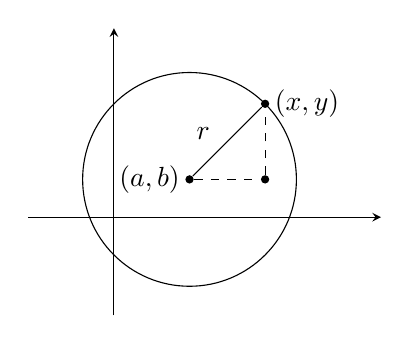
\begin{tikzpicture}
  \begin{axis}[ xmin=-0.1,
    xmax=2.5,
    ymin=-1.3,
    ymax=2.5,
   axis equal,
    axis lines=middle,
 ticks=none,
xlabel={},
ylabel={},
  ]
\node[circle,fill,inner sep=0pt,minimum size=3pt] (P) at (1,0.5) {};
\node[below,left] at (1,0.5) {$(a,b)$};
\node[circle,fill,inner sep=0pt,minimum size=3pt] (Q) at (2,1.5) {};
\node[above,right] at (2,1.5) {$(x,y)$};
\node[circle,fill,inner sep=0pt,minimum size=3pt] (R) at (2,0.5) {};
\draw (P)--(Q);
\draw[dashed] (P)--(R)--(Q);
\node[above,left] at (1.4,1.1) {$r$};
\draw (1,0.5) circle [radius =sqrt(2)]; 
\end{axis}
 \end{tikzpicture}
  \caption{Cirklens ligning.}
  \label{fig:2lec}
\end{figure}
Alle punkterne der ligger på denne cirkel vil opfylde at deres afstand til punktet $(a,b)$ er $r$. Dette kan vi ved hjælp af afstandsformlen skrive som en ligning givet ved
\begin{align*}
(x-a)^2+(y-b)^2=r^2,
\end{align*}
hvor $(x,y)$ er punkter på cirklen. Denne ligning kaldes for \emph{cirklens ligning}.

\paragraph*{Eksempler:}
\begin{enumerate}
\item Find cirklens ligning for en cirkel med centrum i $(2,3)$ med radius $r=4$:

Vi indsætter $(2,3)$ og $r=4$ i cirklens ligning og reducere
\begin{align*}
(x-2)^2+(y-3)^2=16.
\end{align*}
\item Find centrum og radius for en cirkel med ligning $x^2-4x+y^2-2y=-4$:

For a omskrive ligningen til noget på samme form som cirklens ligning vil vi bruge kvadratsætningerne den modsatte vej af hvad vi har gjort indtil nu. Vi ser at 
\begin{align*}
x^2+4-4x &= (x-2)^2 \\
y^2+1-2y &= (y-1)^2.
\end{align*} 
Dermed kan vi, hvis vi lægger $5$ til på begge sider af den givne ligning, omskrive den til
\begin{align*}
x^2-4x+y^2-2y=-4 &\Leftrightarrow x^2-4x+y^2-2y+5=1 \\
& \Leftrightarrow (x^2+4-4x)+(y^2+1-2y)=1 \\
& \Leftrightarrow (x-2)^2+(y-1)^2=1^2,
\end{align*}
hvilket viser at cirklen har centrum i punktet $(2,1)$ og radius $r=1$.
\item Find centrum og radius for en cirkel med ligning $x^2+4x+y^2-4y=1$:

Vi benytter igen kvadratsætningerne den modsatte vej, og får at
\begin{align*}
x^2+4+4x&=(x+2)^2\\
y^2+4-4y&=(y-2)^2.
\end{align*}
Dermed kan vi, hvis vi lægger $8$ til på begge sider af ligningen, få at
\begin{align*}
x^2+4x+y^2-4y = 1 &\Leftrightarrow x^2+4x+y^2-4y +8 = 9 \\
&\Leftrightarrow (x^2 + 4 + 4x) + (y^2 + 4 - 4y) = 9 \\
&\Leftrightarrow (x+2)^2 + (y-2)^2 = 9 \\
&\Leftrightarrow (x-(-2))^2+(y-2)^2 = 3^2,
\end{align*}
\end{enumerate}
hvilket viser at cirklen har centrum i $(-2,2)$ og radius $3$.